\chapter{Introduction}

\section{The Active Galactic Nuclei}
Active galaxies constitute a distinctive class characterized by an intensely energetic source at their center, known as an Active Galactic Nucleus (AGN). Since the first observation of an active galaxy in the early 1900s, numerous studies have been conducted on this intriguing category of galaxies. To this day, efforts persist in unraveling the nature and role of active galaxies within the broader context of galactic formation and evolution.

Research in this field has demonstrated that the intense radiation must emanate from a compact region, with a spatial dimension not exceeding 100 parsecs. This estimation was derived from the temporal variability observed in some of these sources \cite{1959ApJ...130...38W}. Additionally, it has been noted that AGNs exhibit luminosity variations of over $50\%$ within timescales ranging from days to years. Such fluctuations can only be explained if a substantial portion of the emission region is randomly connected. These observations strongly imply that the central component of AGNs is likely a Supermassive Black Hole (SMBH), namely a rapidly accreting black hole.

AGN emissions span the entire electromagnetic spectrum, with variations in the different components depending on the classification of the observed nuclei. Despite these differences in emissions, a General Model known as the "Unified model" can still be defined, which applies to each classification of AGNs. \cite{1995PASP..107..803U}

In addition to the previously mentioned supermassive black hole (SMBH) at the center, there is an accreting disk located in close proximity, serving as a primary source of UV radiation. The central region, excluding the disk, is the main contributor to X-rays, while gas clouds orbiting near the BH give rise to Broad Emission Lines, forming what is known as the Broad Line Region (BLR).
In the outer regions, situated both above and below the accreting disk, the primary contributor to Narrow Emission Lines, thus defining the Narrow Line Region (NLR), is the presence of diffuse gas. Additionally, surrounding the disk, there's a toroidal-shaped volume composed of a mixture of gas and dust, leading to the partial absorption of central radiation.

The final torus-shaped volume is indeed one of the main reasons for explaining the extreme variety observed in active galaxies and the different modes in which SMBH growth occurs. From a historical perspective, AGNs are divided into two main categories: Type 1 and Type 2, with the addition of Blazars. According to the 'Unified Model,' the main difference between these categories is merely apparent, arising from nothing more than variations in the observer's line of sight and the presence of the obscuring torus.

\begin{figure}[b]
  \centering
  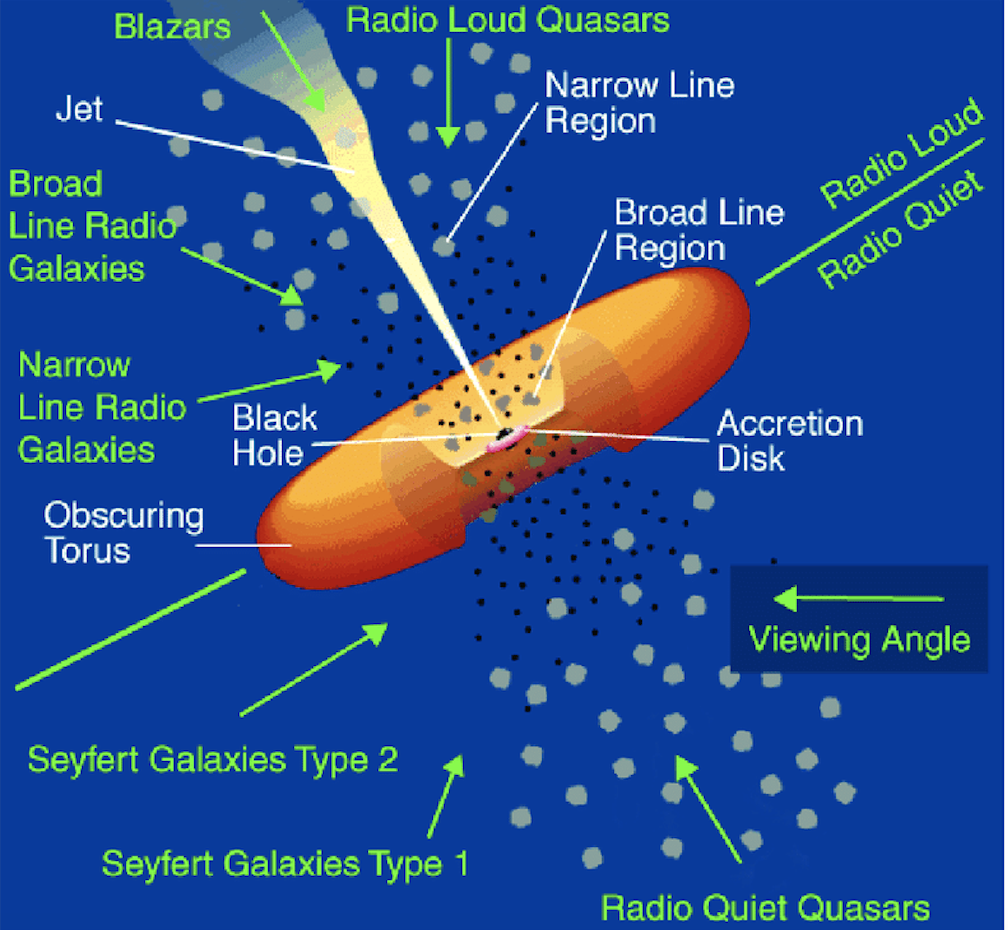
\includegraphics[width=0.55\textwidth]{UnifiedAGNmodel}
  \caption{Fig 2 : Unified AGN model as proposed in \cite{1995PASP..107..803U}}
  \label{2}
\end{figure}


\begin{itemize}
  \item \textbf{Type I:} The emission lines exhibit a broad component, typically in the range of $\sim 10^{3}$-$10^{4}, \text{km s}^{-1}$, along with a narrow component. In this configuration, the observer is situated at a small angle relative to the torus axis, allowing the radiation from circumnuclear regions to remain unobscured along the line of sight
  
  \item \textbf{Type II:} Emission lines exhibit only a narrow component, typically not exceeding $1200 , \text{km s}^{-1}$. In this scenario, the line of sight intersects the obscuring matter of the torus.
  
  \item \textbf{Blazars:} 
\end{itemize}


% RICORDATI DI AGGIUNGERE ANCHE LA PARTE SULLE MODALITA' DI MANIFESTAZIONE DEI QSO : RADIO E OPTICAL 

\newpage
\section{The Brightest Cluster Galaxies }
The Hierarchical model stands as a cornerstone in our understanding of cosmic structure formation, delineating the principal pathways through which galaxies burgeon in both stellar luminosity and mass. At its core, this model elucidates how galaxies amass their content by drawing in and assimilating matter from their surroundings.

One of the most extreme examples in this context involves the study of Brightest Cluster Galaxies (BCGs), a unique class of galaxies, often situated at the center and typically standing out as the most luminous and massive objects within the entire cluster.( e.g. \cite{2015MNRAS.448....2W} ).

Considering their environment, observational studies, such as \cite{2020MNRAS.498.2719T}, have indicated that the evolution of Brightest Cluster Galaxies (BCGs) differs from the normal galactic path. The prevailing model for cosmic structure formation ( i.e. the Cold Dark Matter Model ) suggests that the mass assembly of BCGs is primarily influenced by dry mergers \cite{2007MNRAS.375....2D, 2019ApJ...881..150C}.

At low redshift, these objects exhibit a small dispersion in their aperture luminosities and, indeed, have been frequently chosen as standard candles for cosmological tests throughout the literature, also because of the shared properties with the cluster itself.

Mainly found to be Elliptical galaxies, BCGs seems to not be drawn from the same luminosity function as normal elliptic objects outside the cluster environment, and in general has been proven to differ also from generic Bright galaxies.
 ( i.e. \cite{1977ApJ...212..311T}) 
  
Due to their distinct evolutionary histories, the primary mechanism driving the mass growth of galaxies is associated with cooling flows within lower mass halos at high redshifts. However, at low redshifts, this phenomenon diminishes, primarily due to increased Active Galactic Nuclei ( AGN ) activity accreting mass into their typically hosted SMBH \cite{2006ApJ...652..216R}.
 
As presented before regarding AGN feedback, also BCGs are interested by both of the Quasi Stellar Object modes, resulting in both in the form of Optical AGN, and Radio Loud Emission such as Radio Jets( e.g. \cite{2007MNRAS.379..867V} ).

These relativistic jets of radio emission is also recognized as one of the main explanation of the so called "Cooling flow problem". The unique relaxed and virialized environment defining the cluster often has cooling time-scales much shorter than Hubble time, that following to the absence of a heating source would lead to the presence of a cooling flow.

However observational studies found that temperature of cluster cores fails to fall below $\sim 30\%$ at large radii resulting in an amount of cooling gas corresponding only to the $\sim 10\%$ expected from the existent cooling flow model. \cite{David_2001}

\begin{figure}[t]
  \centering
  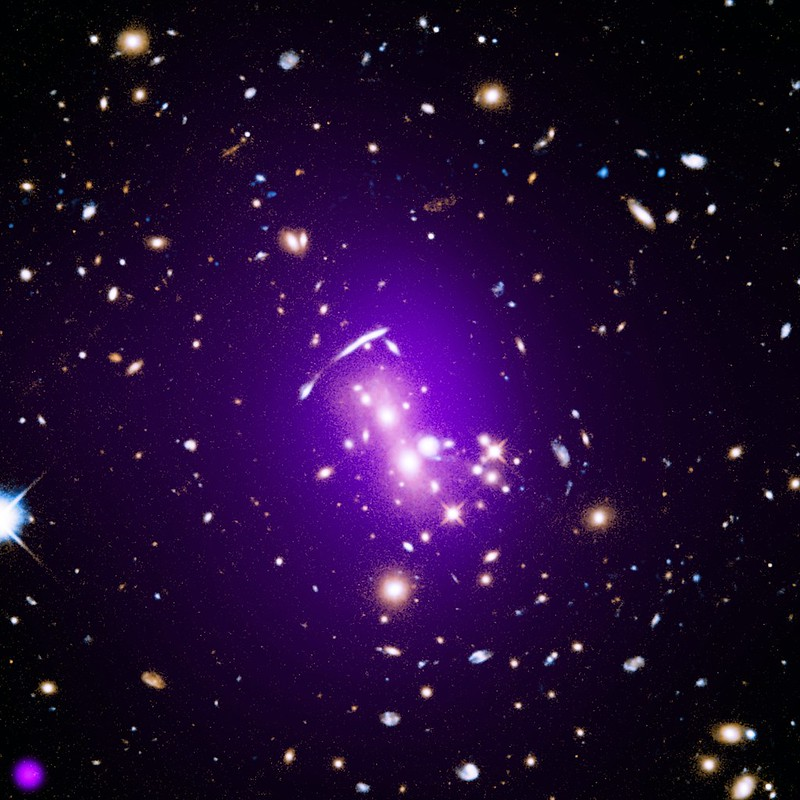
\includegraphics[width=0.5\textwidth]{BCG}
  \caption{This image of galaxy cluster SPT-CLJ0310-464
  X-rays from Chandra are shown along with optical data from Hubble}
  \label{1}
\end{figure}






% Aggiungi parte sulle merging activity
% aggiungi parte su cosa si vede a bassi z e quali sono le teorie in questo senso che tengono banco
% Aggiungi dei riferimenti alle domande che restano aperte nel contesto.



%Thanks to the unique environment in which BCGs are located, made by over-dense 

\section{The Aim of this thesis}

